%% ----------------------------------------------------------------
%% Results.tex
%% 333 ---------------------------------------------------------------- 
\chapter{Results \& Discussion} \label{Chapter: Results}

% Parameters are defined in Results (not in Methods)

% Report is a presentation of the final results, not the whole process.

% Draw inferences from proofs

% Check that your paper is focused. Choose the point of the paper and its key conclusion before you begin writing, stick to your choices, and write the paper so that the reader gets the point already in the abstract and in the introduction. Leave  out results that are not required for supporting the key conclusion, or safely tuck them away in the supplementary information document. When editing, if you feel that your paper loses its focus at some point, take a step back and do a major rewrite.

% Check that there is a clear question and a clear answer—it is all too common to focus on your results and what you have done, instead of stating and then solving a problem. Your results are meaningful only if they solve a meaningful problem. Remember that your paper is neither an account of your work nor a lab diary; it should be a story of an important problem and its solution. Emphasise the problem, both in the Introduction where it should really stand out, and in the Results section and the Discussion. Make it clear to the reader how each result contributes to solving the problem, and what the implications of solving the problem are.

%\begin{enumerate}
%\item What did I find?
%\item Let me describe the best bits
%\item Here is my analysis and proof of it
%\item Here's my conclusion(s) about it
%\end{enumerate}

I have trained the network described in section \ref{sect:network} for 400 epochs with the same parameters as the ones used by \cite{Jurtz2017}; i.e., gradient clipping at 20, regularization term $\lambda=10^{-3}$, and training-validation split at the 5278th sequence. The resulting network reaches an accuracy of 67.7\% on the test set, which is not to far from the 70\% of the state-of-the-art (see section \ref{sect:HoF}). I believe that such a small difference does not undermine the effectiveness of the other results, and furthermore alights the computational burden of a more complicated model.

\section{Outlier analysis} \label{sect:outliers}

In order to analyse the performance space a bit better and, the average accuracy per sequence has also been calculated and shown in Figure \ref{fig:per_seq_acc}. The distribution exhibits the typical funnel shape that one could expect from processes with random variables forming groups of different sizes: the bigger the groups, the smaller the variance. The funnel ceases to shrink at length about 400, so it would be particularly interesting to understand why the network is classifying worse (60\% and below) some of the sequences above that length.

% CHeck alpha-helix size
If we observe the color scheme, we can understand right away that sequences rich in $\alpha$-helix are generally better predicted than $\beta$-sheets and coils. An explanation could be that while $\alpha$-helix sizes are up to CHECK NUMBER, which is inside the window size, $\beta$-sheets interact with amino-aids further away in the sequence, which is not possible to be captured with the window of the network, of lateral size of 9.

\begin{figure}
\centering
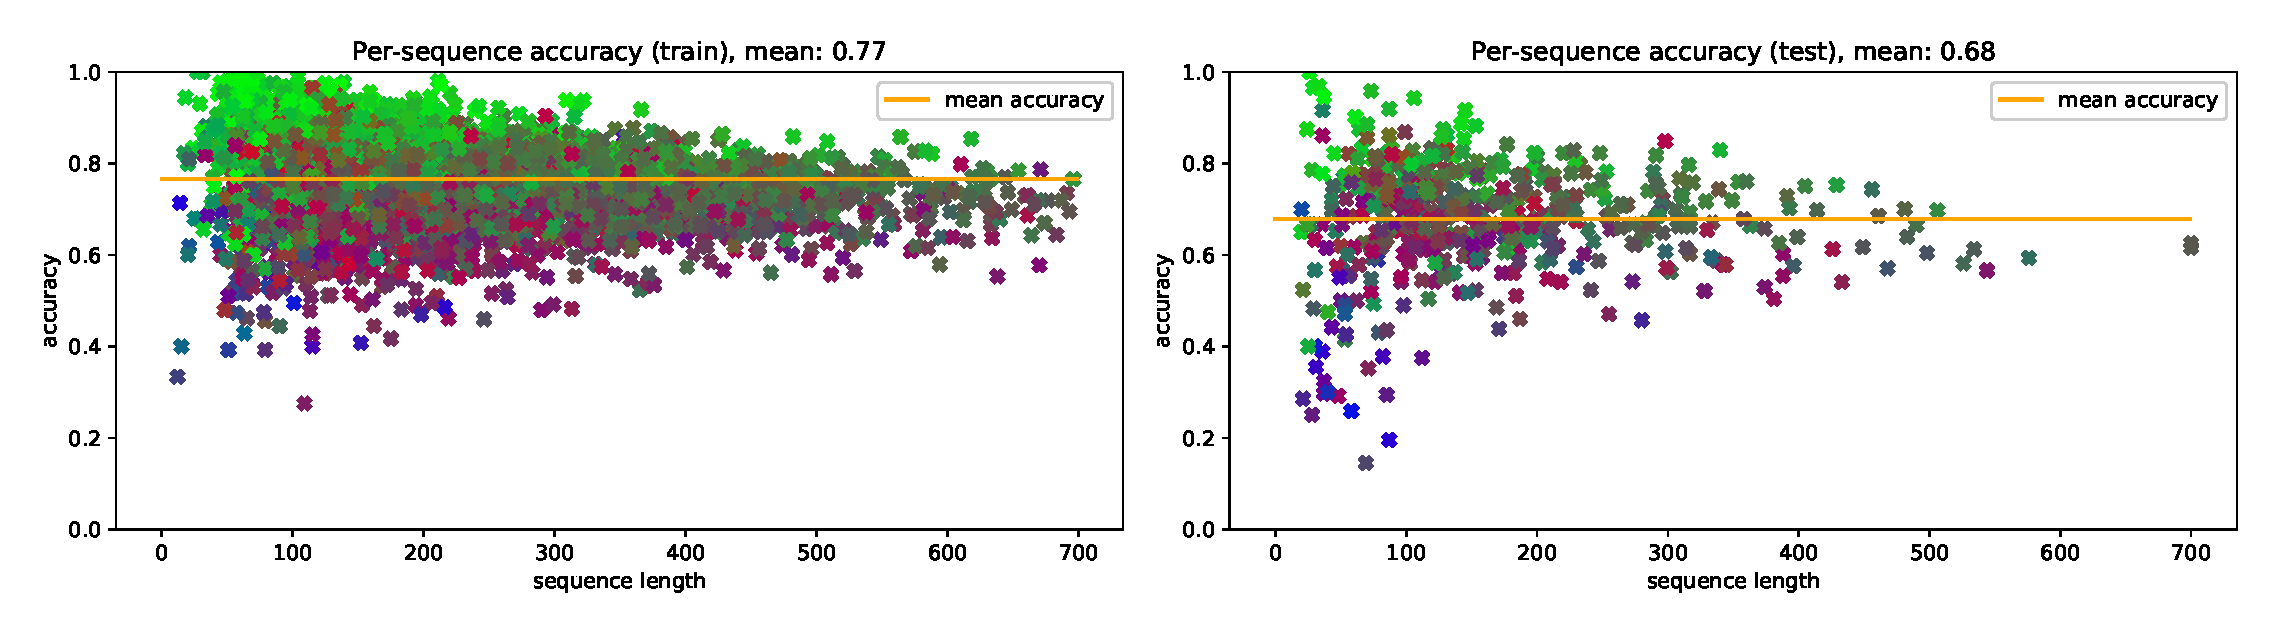
\includegraphics[width=1\linewidth]{Figures/per_seq_acc}
\caption{The mean accuracy per sequence by sequence length. The 5504 sequences of the training set are shown on the left and the 514 of the test set on the right. Each point represents a single protein, and its colour corresponds to the amount of $\beta$-sheet (red), $\alpha$-helix (green), and coils (blue) it has. A purple point, for instance, would predominantly have $\beta$-sheets and coils.}
\label{fig:per_seq_acc}
\end{figure}
% EXtra: include the same graph but colour the high-appearing classes and the low appearing classes differently (RB)

\section{Feature visualization}

	\subsection{First layer filters}
	
	\subsection{Saliency maps on layers?}


\section{Saliency maps on inputs}
Talk about dimensions: saliency value, class, sequences, positions, window, amino-acids, aa/pssm (7 dimensions). From now on, individual saliency maps will refer to the saliency map of one sequence-position

Options (all options could be applied either to aa or to pssm, 6 dimensions left)
% PRove that saliencies on pssm are much more powerful than saliencies on aas
One way to prove it is to show that for every single position, the (addition / maximum after aggregated by window but not by class) of pssm saliencies is bigger than the (addition / maximum etc) of aas saliencies
	
	\subsection{Saliency maps on single sample sequences}
	% SHow per-class samples of this instances (either graph form, SeqLogo form) (either per-position or heat-map)
	analyse per-class single sequence (sample-based) (4 dimensions left): aa-aggregated (3 dimensions) and added in the sequence position, either respecting each position (3 dimensions) or aggregating them in a heat map (2 dimensions), or aggregating the positions in a heatmap but containing the 8 classes (3 dimensions) (Colour the labels with the RGB either form Figure \ref{fig:per_seq_acc} or with the colour code from \ref{sect:sheer}).
	
	Have the x labels including amino-acid, prediction, and real label. Colour classes with the codes mentioned in the previous paragraph. Consider marking mismatches in bold.
	
	Have as the sample one of the sequences with low accuracy and high length from \ref{sect:outliers}

	\subsection{Sheer addition} \label{sect:sheer}
	aggregate all individual saliency maps % SHould I try to compare my results with known motifs? Absolutely yes!
	sheer addition (4 dimensions left): class-aggregated (3 dimensions), aa-aggregated (3 dimensions), or class+aa-aggregated (2 dimensions)
		\subsubsection{Per-aminoacid and class aggregations}
		% INclude per-class aggregations (absolute value, aa aggregated) -> class profile (flatness, distribution, etc)
		% XAxis labels should be centered on 0 and going to +-9
		
		\subsubsection{Per-class aggregations}
		% INCLUDE per-class aggregations (either graph form, SeqLogo form, or both). Include just a few and leave the others as supplementary materials.
		First thing to notice: pssm is way more relevant than one-hot encoded aas. No wonder, it learns faster.

		\subsubsection{Per-aminoacid aggregations}
		% INclude per-aminoacid aggregations? (Same, just a few and the others as supplementary)

	\subsection{Clustering techniques}
	aggregate all individual saliency maps % SHould I try to compare my results with known motifs? Absolutely yes!
	clustering (5 dimensions left)
	Using the per-class window-aggregated version of individual saliency maps (4 dimensions left)
	Cosine distance metric.
	Show either all profiles per-cluster (3 dimensions), or aggregated profiles (2 dimensions)
	Show t-SNE with points coloured by cluster
